%%%%%%%%%%%%%%%%%%%%%%%%%%%%%%%%%%%%%%%%%%%%%%%%%%%
%% Capítulo 2: Iteración
%%%%%%%%%%%%%%%%%%%%%%%%%%%%%%%%%%%%%%%%%%%%%%%%%%%

Como hemos podido comprobar en el capítulo anterior, muchos de los fractales clásicos son generados repitiendo indefinidamente un proceso. Iteración es el proceso de repetir una y otra vez un método, ocasionalmente sobre el resultado de la aplicación anterior. Este procedimiento es muy útil en muchas disciplinas matemáticas. Por ejemplo, existen métodos numéricos basados en la iteración como el método de \textit{Jacobi} y \textit{Gauss-Seidel} para resolución de sistemas de ecuaciones lineales, el método de \textit{Newton-Raphson} para encontrar soluciones de ecuaciones, el método de \textit{Runge-Kutta} para resolución numérica de ecuaciones diferenciales, etc. Incluso en otras disciplinas como el aprendizaje automático los algoritmos de \textit{K-Means} para ``clustering'' o los métodos de generación de árboles de decisión en problemas de clasificación hacen uso de procesos iterativos. Esta metodología aplicada sobre el plano complejo y sobre ciertas funciones complejas será la que nos proporcionará nuestros primeros ejemplos de imágenes fractales.

\section{Iteración de funciones}
\begin{definicion}
    Consideramos una función $f:\C\longrightarrow\C$ y un punto $z\in\C$. La aplicación sucesiva de $f$ a $z$ -- \textit{i.e.} $z,f(z),f(f(z)), f(f(f(z))),\dots$ -- produce las \textit{iteradas} de la función $f$ en el punto $z$. Al conjunto de dichas iteradas se le denomina \textit{órbita} $O_f(z)$ de $f$ en $z$.
    $$
    O_f(z):=\left\lbrace z, f(z), f^2(z), \dots, f^n(z), \dots\right\rbrace.
    $$
    donde $f^n$ denota a $f\circ f^{n-1}$.
\end{definicion}

Lo siguiente es plantearse la posible convergencia de la sucesión $\{f^n(z)\}$. Para ello, y a partir de este momento nos ayudaremos del software \textcolor{blue}{\href{https://www.wolfram.com/mathematica/}{Mathematica®}} en su versión 12 (concretamente la versión 12.1)\footnote{Los códigos completos que generan cada una de las imágenes que se observan en este documento se pueden encontrar en \url{https://github.com/JAntonioVR/Geometria-Fractal/tree/main/Iteracion-y-Fractales}}. El comando \verb|NestList[f,z,n]| itera una función \verb|f|, comenzando en el punto \verb|z| un total de \verb|n| veces y devuelve una lista con los \verb|n| valores. 

Para saber qué ocurre a largo plazo podemos iterar un número grande de veces, fijémonos lo que ocurre si utilizamos $f(z):=z^2$ comenzando por $z_0=0.9$.

\begin{verbatim}
In[]:= f[z_] = z^2;
    NestList[f, 0.9, 10]
    
Out[10]= {0.9, 0.81, 0.6561, 0.430467, 0.185302, 0.0343368,
    0.00117902, 1.39008*10^-6, 1.93233*10^-12, 3.73392*10^-24, 
    1.39421*10^-47}
\end{verbatim}

Como se puede observar, en cada iteración se acerca cada vez más a $0$, lo cual denotamos con $\{f^n(0.9)\}\rightarrow 0$. Nuestro objetivo ahora es poder conocer el comportamiento de la órbita de una función y un punto dados. 

\subsection{Tipos de convergencia}

Fijémonos que en el ejemplo anterior si en lugar de tomar $z_0=0.9$ hubiésemos tomado cualquier valor con $|z_0|<1$ la convergencia habría sido igualmente a $0$, pues elevamos al cuadrado cada vez números más pequeños. Justo al contrario ocurre si $|z_0|>1$, en cuyo caso la sucesión diverge. Por último, en caso de que $|z_0|=1$, esto es, $z_0\in S^1$, la sucesión $\{f^n(z_0)\}$ nunca saldrá de $S^1$, siendo este el conjunto que delimita la frontera entre el conjunto de puntos cuya sucesión converge o diverge. En particular, $f^n(-1)=f^n(1)=1\ \ \forall n\in\N$, por lo que $z=1$ es un punto fijo de $f$, es decir, $f(z)=z$. 

Nos interesa particularmente saber qué sucesiones de iteradas convergen y a qué elemento convergen. En este sentido \textit{Stephan Banach} demostró uno de los resultados más útiles y vigentes del análisis funcional:

\begin{teorema}[Punto fijo de Banach]
    Sea $X$ un espacio métrico completo y $f:X\longrightarrow X$ una aplicación contractiva. Entonces $f$ tiene un único punto fijo. Además, la sucesión de iteradas $\{f^n(x_0)\}$ converge a dicho punto fijo para cualquier $x_0\in X$. 
\end{teorema}
\begin{proof}
    Probaremos primero la existencia:

    Sea $x_0\in X$ y sea la sucesión de iteradas $\{x_n\}=\{f^n(x_0)\}$. Por ser $f$ contractiva, llamamos $K<1$ a su constante de Lipschitz. Probaremos por inducción que $d(x_n,x_{n+1})\leq K^n d(x_0,x_1) \ \ \forall n\in\N$.
    El caso base es cierto pues $d(x_1,x_2)=d(f(x_0),f(x_1))\leq K d(x_0,x_1)$. Si suponemos que la hipótesis es cierta para cierto $n$, tenemos que
    $$
    d(x_{n+1},x_{n+2})=d(f(x_n),f(x_{n+1}))\leq K d(x_n,x_{n+1})\leq K^{n+1}d(x_0,x_1).
    $$
    Ahora, para $n,r\in\N$:
    \begin{eqnarray*}
        d(x_n,x_{n+r}) & \leq & \sum_{j=0}^{r-1}d(x_{n+j},x_{n+j+1}) \leq d(x_1,x_0)\sum_{j=0}^{r-1}K^{n+j} \leq K^n d(x_0,x_1)\sum_{j=0}^{\infty} K^j \\
        & = & \frac{d(x_0,x_1)K^n}{1-K}.
    \end{eqnarray*}
    Dado $\varepsilon>0$, como $\{K^n\}\rightarrow 0$, existe un $m\in\N$ tal que para $n>m$ se tiene que $d(x_0,x_1)K^n<\varepsilon(1-K)$. Si ahora tomamos dos naturales $p,q\geq m$ con $p<q$, aplicando la desigualdad anterior tomando $n=p$ y $r=q-p$ obtenemos que:
    $$
    d(x_p,x_q) = d(x_n, x_{n+r}) \leq \frac{d(x_0,x_1)K^n}{1-K} < \varepsilon
    $$
    de donde deducimos que $\{x_n\}$ es una sucesión de Cauchy, y como $X$ es completo, tenemos que $\{x_{n+1}\}=\{f(x_n)\}=\{f^n(x_0)\}\rightarrow x\in X$. Pero $f$ es continua, por lo que si $\{x_n\}\rightarrow x$, necesariamente $\{f(x_n)\}\rightarrow f(x)$, por lo que $f(x)=x$.

    Para probar la unicidad, suponemos que $y\in X$ es otro punto fijo de $f$, por lo que $d(x,y) = d(f(x),f(y))\leq K d(x,y)$. Tomando el primero y el tercer miembro de la desigualdad deducimos que $(1-K)d(x,y)\leq 0$, luego $d(x,y)=0$.
\end{proof}

Este teorema unido a que sabemos que $\C$, y por tanto todos sus subconjuntos cerrados, es completo, nos permite asegurar convergencia de las sucesiones $f^n(x_0)$ a un punto fijo para cualquier $x_0$.




\subsection{Velocidad de convergencia}

En estos casos, han sido suficientes 20 iteraciones para conocer el comportamiento de la órbita a largo plazo, pero interesa saber cuántas iteraciones son necesarias en cada punto para saber si hemos alcanzado el valor al que converge la sucesión. Este alcance se toma como aproximado, pues generalmente nunca se llega a alcanzar el punto fijo, tan solo podemos reducir la diferencia tanto como queramos. En este sentido, \textit{Mathematica} tiene dos comandos útiles:

\begin{itemize}
    \item \verb|FixedPointList[f,expr]| genera una lista de valores resultantes de aplicar \verb|f| a \verb|expr| repetidamente hasta que los dos últimos valores no cambian. Para parametrizar la precisión en la proximidad de los valores podemos utilizar el argumento opcional \verb|SameTest|\footnote{Más información en la documentación oficial \url{https://reference.wolfram.com/language/ref/FixedPointList.html}}.
    \item \verb|FixedPoint[f,expr]| hace lo mismo pero produce como salida únicamente el valor último producido.
\end{itemize}

El siguiente código muestra un ejemplo de uso:

\begin{verbatim}
In[]:= f[x_] = x/2 + 1/x;
    FixedPointList[f, 1.0, SameTest -> (Abs[#1 - #2] < 10^-4 &)]
    FixedPoint[f, 1.0]

Out[]= {1., 1.5, 1.41667, 1.41422, 1.41421}
Out[]= 1.41421
\end{verbatim}

Y a partir de la longitud de la lista que nos devuelve \verb|FixedPointList|, es decir, con el sencillo comando \verb|Length[FixedPoint[f,x]]| podemos medir la velocidad de convergencia de cada punto.

\section{Iteración en $\C$}

De manera natural, todos los conceptos explicados anteriormente sobre iteración en $\R$ se pueden extender al plano complejo. Esto es, dada una función compleja $f:\C\longrightarrow\C$ y un número complejo $z\in\C$, podemos preguntarnos por el comportamiento a largo plazo de la órbita $O_f(z)$. En este caso, y utilizando la correspondencia entre un punto $(x,y)\in\R^2$ y un número complejo $z=x+i\cdot y$, podemos representar cada punto de una órbita como un punto del plano, pudiendo así fácilmente graficar las órbitas y observar su comportamiento. Observamos en la imagen \ref{fig:orbitas-C} dos ejemplos de esto, ambos han sido generados por el código siguiente, cambiando necesariamente los parámetros para generar la figura (b), de aspecto más armónico.

\begin{verbatim}
In[]:= f[z_] := z^2;
    x0 = 0.9 + 0.3 I;
    ComplexListPlot[N[FixedPointList[f, x0, 10]]];
    ComplexListPlot[N[FixedPointList[f, x0, 10]], Joined -> True];
    Show[%, %%]
\end{verbatim}

\begin{figure}[h]
    \begin{tabular}{cc}
      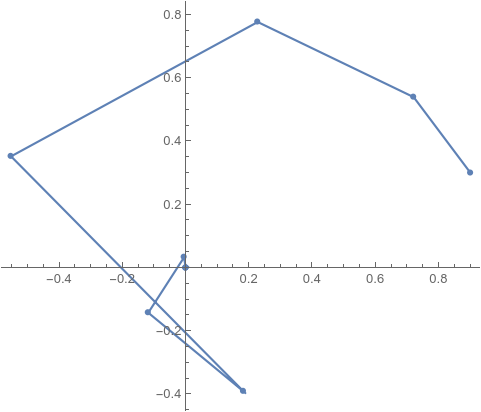
\includegraphics[scale=0.45]{./img/orbita-1.png} &   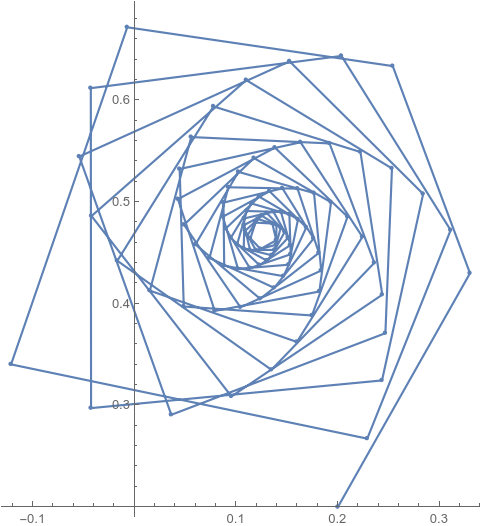
\includegraphics[scale=0.4]{./img/orbita-2.png} \\
    (a)$f(z)=z^2$ en $z=0.9+0.3i$ & (b) $f(z)=z^2+0.33+0.35$ en $z=0.2+0.2i$ \\[6pt]
    \end{tabular}
    \caption{Representación de dos órbitas en $\C$}
    \label{fig:orbitas-C}
\end{figure}

De hecho, para la función $f(z)=z^2$ se tiene que la órbita de todo $z$ con módulo $|z|<1$ tiende a $0$, mientras que si $|z|>1$ diverge y si $|z|=1$ su órbita permanece siempre en la esfera unidad $S^1$. Por tanto, $S^1$ se convierte en la frontera entre los puntos \textit{de escape} -- cuyas órbitas escapan -- y los puntos \textit{prisioneros} -- cuyas órbiras convergen. Por tanto los puntos del plano complejo presentan una dicotomía para la función $f$: escapar o no. $S^1$, al ser la frontera entre estos dos conjuntos, es conocido como el \textit{conjunto de Julia} de la función $f(z)=z^2$. Esta idea será tratada detenidamente en el capítulo \ref{chap:Julia-Mandelbrot}.

\section{El método de Newton y cuencas de atracción}

La iteración es la base de muchos métodos numéricos, entre los que en este caso destacamos el `método de Newton', el cual fue inicialmente descrito por \textit{Isaac Newton} en su libro \textit{De analysi per aequationes numero terminorum infinitas}. Este es un procedimiento muy útil y utilizado en la resolución numérica de ecuaciones, tratando buscar con cierta precisión el punto en el que se anula una función $f:\R\longrightarrow\R$, aunque gracias al trabajo de \textit{Arthur Cayley} sabemos que es posible generalizarlo a los números complejos.

Recordemos que dada una ecuación $f(z)=0$ para cierta función compleja y derivable $f:\C\longrightarrow\C$, el método de Newton itera la función
\begin{equation}
    \label{eq:metodo-Newton}
    N_f(z)=z-\frac{f(z)}{f'(z)}
\end{equation} 
comenzando por un punto $z_0$ cercano a la raíz. Es decir, calcula la sucesión $\{z_n\}$ definida como $z_{n+1}=N_f(z_n) \ \forall n\in\N$, la cual converge a un punto $a\in\C$ que verifica $f(a)=0$.

Sin embargo, en muchas ecuaciones, comenzando por las polinómicas de grado mayor que 1, existen varias soluciones distintas, pero el método de Newton converge sólo a una de ellas, dependiendo de qué $z_0$ fijemos. Nuestro objetivo ahora se sitúa en discernir, para cada punto $z_0$ del plano, a qué solución de la ecuación $f(z)=0$ converge la sucesión $\{z_n\}$ dada por el método de Newton utilizando a $z_0$ como semilla. En las siguientes secciones veremos algunos ejemplos de esta distinción y su utilidad, llegando a las primeras imágenes fractales generadas por iteración.

\subsection{Caso $z^2-1$}
\label{subsection:cuencas-1}

Consideramos la función compleja $f:\C\longrightarrow\C$ dada por $f(z)=z^2-1$, la cual tiene dos raíces: $1$ y $-1$, las dos raíces cuadradas de 1. Una forma sencilla de comprobar a qué raíz converge cada sucesión utilizando como semilla cada $z_0\in\C$ es asociando un color a cada punto del plano dependiendo de la raíz a la que converja y pidiendo a \textit{Mathematica} que coloree el plano complejo siguiendo este criterio.

\begin{verbatim}
In[]:= iteracionN = #2 - #1[#2]/Derivative[1][#1][#2] &;
    newtonArgumento = 
      Compile[{{z, _Complex}}, 
       Arg[FixedPoint[iteracionNR[f, #] &, z, 50]]];
    
In[]:= DensityPlot[newtonArgumento[x + I*y], {x, -2, 2}, {y, -2, 2}, 
     PlotPoints -> 100, Mesh -> False, ColorFunction -> "Rainbow"] 
\end{verbatim}

\begin{figure} [h]
\centering
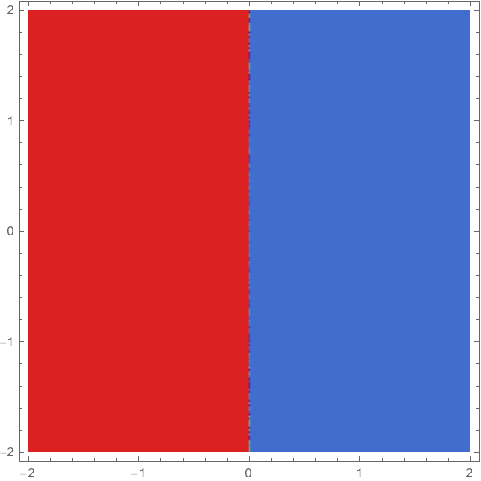
\includegraphics[scale = 0.4]{img/cuencas-1.png}
\caption{Cuencas de atracción de $f(z)=z^2-1$.}
    \label{fig:cuencas-1}
\end{figure}

Produciendo como resultado la imagen \ref{fig:cuencas-1}. La forma de deducir a qué raíz converge cada sucesión consiste en evaluar los argumentos de los valores a los que se acerca la sucesión. Como podemos ver, y teniendo en cuenta que la imagen solo grafica el intervalo $[-2,2]\times[-2,2]$ y un número finito de puntos\footnote{El número de puntos que se grafica se puede parametrizar con el argumento opcional ``PlotPoints'' de las funciones ``Plot''. A mayor valor mayor calidad de imagen y resolución, pero mayor tiempo de ejecución.} la sucesión cuya semilla es un punto perteneciente al semiplano abierto de la derecha converge a la raíz $1$. Por otro lado, si la sucesión comienza con un complejo del semiplano abierto de la izquierda, entonces esta converge a la raíz $-1$. Apoyándonos en este ejemplo, definimos el siguiente concepto.

\begin{definicion}[Cuenca de atracción]
    Definimos como \textit{cuenca de atracción} de una raíz $a\in\C$ de una función compleja $f:\C\longrightarrow\C$ (\textit{i.e.} $f(a)=0$), y denotamos como $A(a)$ al conjunto de puntos $z_0\in\C$ tales que la sucesión $\{z_n\}$ dada por $z_{n+1}=N_f(z_n)$ converge a $a$ utilizando a $z_0$ como primer valor de la sucesión. 
\end{definicion}

Es decir, tenemos en este caso que
$$
A(-1)=\{z\in\C:\operatorname{Re}z<0\},
$$
$$
A(1)=\{z\in\C:\operatorname{Re} z>0\}
$$
y sin embargo los puntos del eje $Y$ no convergen a ninguna de las raíces, siendo esta por tanto la frontera entre las dos cuencas de atracción y el conjunto invariante para $N_f$.

\subsection{Caso $z^3-1$}

Consideremos ahora la función compleja $f:\C\longrightarrow\C$ definida como $f(z)=z^3-1$, cuyas raíces son las raíces cúbicas de 1, es decir: $1, -\frac{1}{2}+\frac{\sqrt{3}}{2}i$ y $-\frac{1}{2}-\frac{\sqrt{3}}{2}i$. De nuevo seguimos la estrategia que hemos tomado en la sección \ref{subsection:cuencas-1}, dividir en píxeles una región del plano complejo y colorear dichos píxeles según distintos colores dependiendo de cuál sea su cuenca de atracción. De esta forma, cada cuenca de atracción será caracterizada por un único color. \textit{Mathematica} permite personalizar la función de color que se utiliza en estos gráficos, de forma que no solo es posible asociar un color, sino una tonalidad de gris mediante el uso del argumento \verb|ColorFunction|, asociandole el valor ``Rainbow", ``Graylevel", o personalizando nosotros mismos la función de coloreado, como veremos más adelante.

\begin{figure}[h]
    \begin{tabular}{cc}
      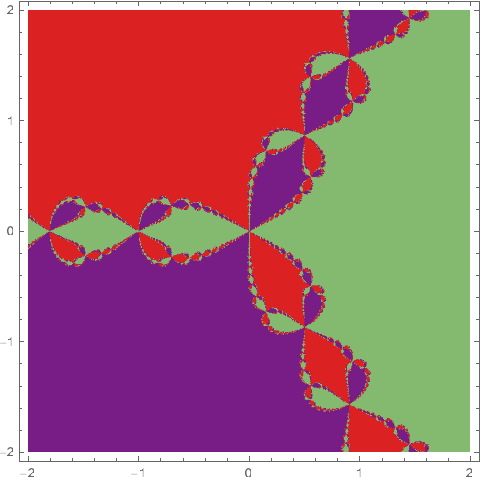
\includegraphics[scale=0.5]{./img/cuencas-2.png} &   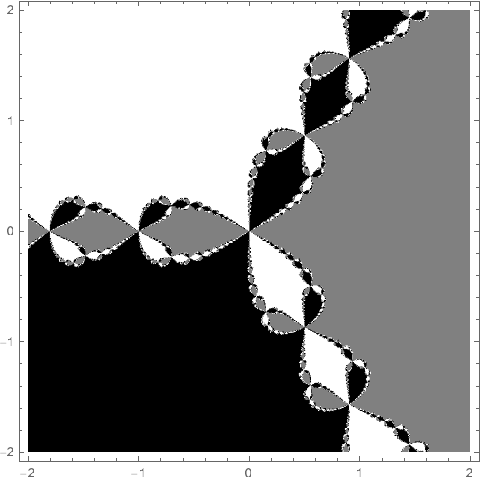
\includegraphics[scale=0.5]{./img/cuencas-3.png} \\
    (a) De colores & (b) En escala de grises \\[6pt]
    \end{tabular}
    \caption{Cuencas de atracción de $f(z)=z^3-1$}
    \label{fig:cuencas-2}
\end{figure}

El resultado de este cálculo es el que se representa en las imagenes \ref{fig:cuencas-2}, que son realmente la misma con coloreado distinto. En estas imágenes podemos ahora sí ver el primer ejemplo de estructura fractal producido por la iteración. Observemos que las sucesiones de dos puntos muy próximos pueden converger a raíces distintas, por lo que este es un ejemplo de \textit{caos matemático}: pequeñas variaciones en las condiciones iniciales conducen a comportamientos muy diferentes.

Otra posibilidad para representar estas imágenes es, en lugar de asociar un color a cada número complejo según la cuenca de atracción a la que perteneciente, evaluar la velocidad de convergencia, es decir, las iteraciones necesarias hasta alcanzar la raíz en cuestión. A partir de esa velocidad de convergencia asignamos un color más o menos intenso. El código necesario se muestra a continuación y el resultado en la imagen \ref{fig:cuencas-velocidad}.

\begin{verbatim}
newtonVelocidad = 
  Compile[{{z, _Complex}}, 
    Length[FixedPointList[iteracionN[f, #] &, z, 50]]];

DensityPlot[newtonVelocidad[x + I*y], {x, -2, 2}, {y, -2, 2}, 
  PlotPoints -> 200, Mesh -> False, ColorFunction -> GrayLevel]
\end{verbatim}

\begin{figure} [h]
\centering
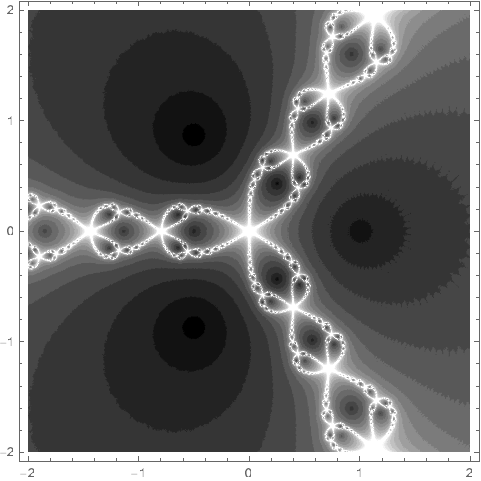
\includegraphics[scale = 0.5]{img/cuencas-velocidad.png}
\caption{Evaluación de la velocidad de convergencia a las raíces.}
    \label{fig:cuencas-velocidad}
\end{figure}

Fijémonos además que si hacemos \textit{zoom} en ciertas partes de la imagen, es decir, representamos una región más pequeña, encontramos estructuras que son iguales independientemente del zoom que se aplique. En la figura \ref{fig:detalles} podemos ver distintos detalles de la figura \ref{fig:cuencas-velocidad}, cada una es una ampliación de la anterior, y podemos ver como esa estructura se repite en todas las escalas.

%\newpage

\begin{figure}[h]
    \begin{tabular}{ccc}
      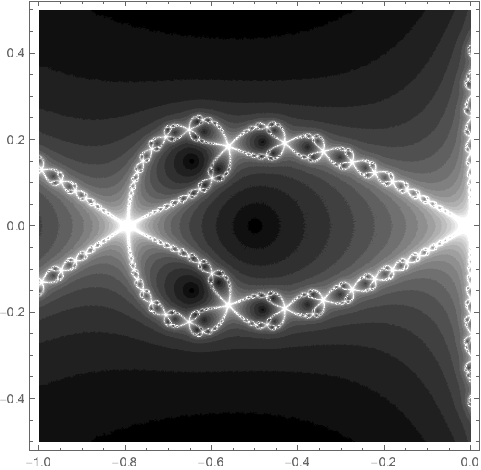
\includegraphics[scale=0.33]{./img/detalle-1.png} &   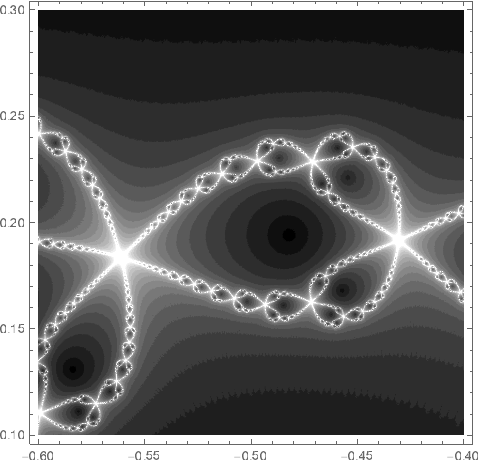
\includegraphics[scale=0.33]{./img/detalle-2.png} &   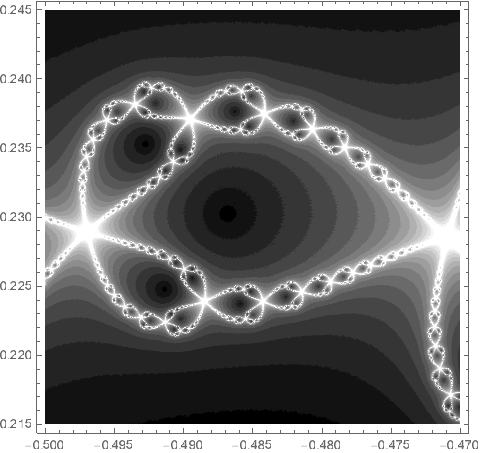
\includegraphics[scale=0.33]{./img/detalle-3.png} \\
    (a) $[-1,0]\times[-0.5,0.5]$ & (b) $[-0.6,-0.4]\times[0.1,0.3]$ & (c) $[-0.5,-0.47]\times[0.215,0.245]$ \\[6pt]
    \end{tabular}
    \caption{Diferentes regiones ampliadas de la figura \ref{fig:cuencas-velocidad}}
    \label{fig:detalles}
\end{figure}

De manera natural, podemos aplicar esta misma teoría a cualquier otro tipo de funciones, como por ejemplo $z^n-1 (n\in\N\backslash\{0,1\})$, o incluso no polinómicas como $z^3-3^z$ o $z^2-2^z-1$ (véanse las imágenes \ref{fig:imagenes-finales}).

\newpage

\begin{figure}[h]
    \centering
    \begin{tabular}{cc}
    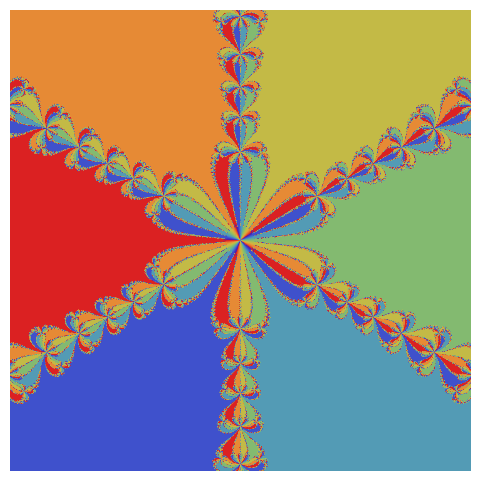
\includegraphics[scale=0.5]{./img/cuencas-4.png} &   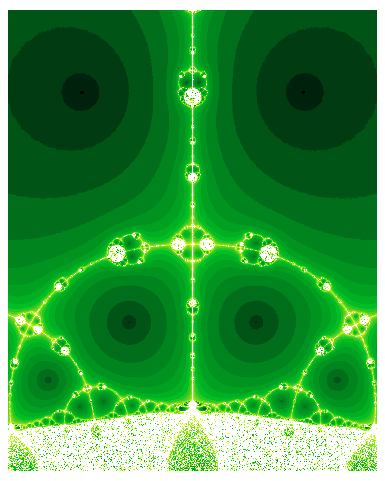
\includegraphics[scale=0.375]{./img/cuencas-5.png} \\
    (a) Función $z^6-1$ & (b) Función $z^3-3^z$ \\[6pt]
    \multicolumn{2}{c}{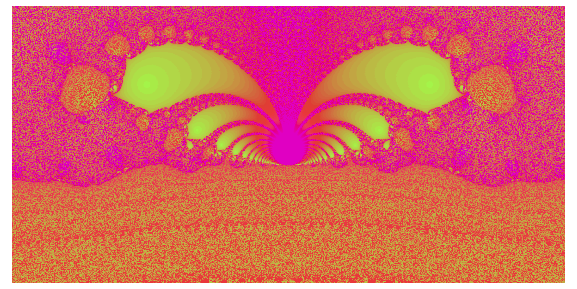
\includegraphics[scale=0.4]{./img/cuencas-6.png}} \\
    \multicolumn{2}{c}{(c) Función $z^2-2^z-1$} \\
    \multicolumn{2}{c}{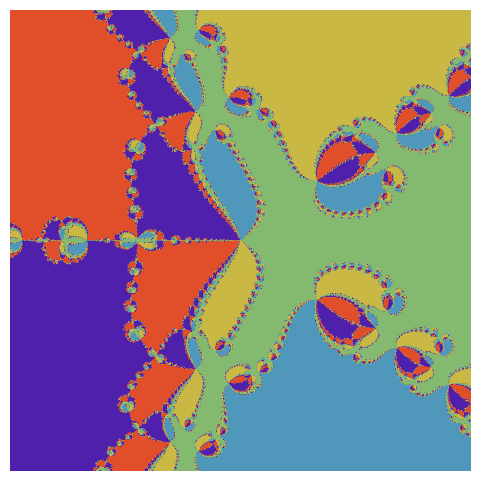
\includegraphics[scale=0.4]{./img/cuencas-7.png}} \\
    \multicolumn{2}{c}{(d) Función $z^5 - z^3 + z^2 - 4$} \\ 
    \end{tabular}
    \caption{Representaciones de cuencas de atracción de distintas funciones.}
    \label{fig:imagenes-finales}
\end{figure}